\documentclass[tikz,border=4pt]{standalone}
\usepackage{tikz}
\usetikzlibrary{arrows.meta}
\begin{document}
\begin{tikzpicture}[>=Stealth]
    \node[font=\bfseries] at (4,4.5) {KL Divergence $D_{KL}(P\|Q)$};

    % Axes
    \draw[->,gray!50] (-0.5,0) -- (8.5,0) node[right,font=\small] {$x$};
    \draw[->,gray!50] (0,-0.3) -- (0,4.2) node[above,font=\small] {$p(x)$};

    % P distribution (blue)
    \draw[blue!70,line width=1.5pt,domain=0.5:7.5,samples=80]
        plot ({\x},{3.8*exp(-(\x-3.5)*(\x-3.5)/1.2)});
    \node[blue!70,font=\bfseries] at (2,3.5) {$P$};

    % Q distribution (red, shifted)
    \draw[red!60,line width=1.5pt,dashed,domain=0.5:7.5,samples=80]
        plot ({\x},{3.2*exp(-(\x-5)*\x-5)/2)});
    \node[red!60,font=\bfseries] at (6.5,3) {$Q$};

    % Arrow showing divergence
    \draw[<->,orange!80!black,line width=1pt] (3.5,1) -- (5,1)
        node[midway,below,font=\small] {divergence};

    % Formula
    \node[font=\small,anchor=north] at (4,-0.4)
        {$D_{KL}(P\|Q) = \sum_x P(x)\log\dfrac{P(x)}{Q(x)} \ge 0$};
\end{tikzpicture}
\end{document}
